\subsection{Eigenvalue Problems - Chapter 27}

\begin{enumerate}

\item {\bf Error Propagation in Euler's Method}
  
  Recall that Euler's method is first order thus Euler's
  method assumes that the first derivative is
  linear in between timesteps. For high order systems, this is not
  necessarily the case. Let us return to the equation for
  $f_2$. In many systems the derivative is simply $\dot{f} =
  af$. Using this result the equation for $f_2$ simplifies to

  \begin{equation}
    f_2 \approx f_1 (1 +a\Delta t)
  \end{equation}

  Similarly 

  \begin{equation} 
    f_3 \approx f_2 (1 +a\Delta t)
  \end{equation}

  Substituting $f_2$ into this equation reduces $f_3$ to

  \begin{equation}
    f_3 \approx f_1 (1+a\Delta t)^2
  \end{equation}
  
  There is a pattern here. 

  \begin{equation}
    f_N \approx f_1 (1+a\Delta t)^{N-1}
  \end{equation}

  This equation is the stability criterion for Euler's method. It
  says that if $|1+a\Delta t|>1$ the system will blow up and
  tend to infinity. Thus, not only will the system not converge
  but it won't even be bounded. Thus care must be taken to choose
  a timestep small enough to ensure that this value is less than
  1. Try simulating $\dot{v} = -2 v$ to see the affect of the
  timestep. 

\item {\bf Application to Differential Equations}

  Euler's method has a unique property in that it convertes a continuous
  differential equation such as the one below  

  \begin{equation}
    \ddot{y} + 2\dot{y} + 4y = 0
  \end{equation}

  into a discrete differential equation like the form below.

  \begin{equation}
    \begin{matrix}
      {y}_{n+1} = {y}_n + \dot{y}_n\Delta t \\
      \dot{y}_{n+1} = \dot{y}_n + (-2\dot{y}_n - 4y)\Delta t
    \end{matrix}
  \end{equation}

  We've done this problem a
  million times but what we haven't done is placed Euler's method into
  the following form. 

  \begin{equation}
    \begin{Bmatrix}
      y_{n+1} \\ \dot{y}_{n+1} \end{Bmatrix} = \begin{bmatrix} 1 & \Delta t
      \\ -4\Delta t & (1-2\Delta t) \end{bmatrix} \begin{Bmatrix} y_{n}
      \\ \dot{y}_n \end{Bmatrix}
  \end{equation}

  In this form it is possible to use vector algebra to compute the
  solution to the differential equation. 
  \begin{equation}
    \vec{y}_{n+1} = A\vec{y}_n
  \end{equation}
  the solution to the differential equation is simply
  \begin{equation}
    \vec{y}_{k} = A^k\vec{y}_0
  \end{equation}
  An interesting result is to compute the stability of Euler's
  method. In order to do that we decompose the matrix A into the
  eigenvalue, eigenvector form $A=V \Lambda V^{-1}$. It is easy to show
  that $A^k = V \Lambda^k V^{-1}$. Furthermore, the computation of
  $\Lambda^k$ is 
  \begin{equation}
    \Lambda^{k} = \begin{bmatrix} {\lambda_1}^k & 0 \\ 0 & {\lambda_2}^k \end{bmatrix}
  \end{equation}
  What you should immediately notice is that if the eigenvalues of the
  matrix A are bigger than one, Euler's method will not converge.

  \item {\bf Solution to ODEs using Eigenvalues}

    It is possible to use matrices and eigenvalues to solve ODEs. Take
    for instance a penduluum with 1 degree of freedom. This system is
    second order as given by the equation below:
    
    \begin{equation}\label{e:full2}
      mL^2\ddot{\theta} + mgLsin(\theta) = 0
    \end{equation}

    In order to solve this equation you need two initial conditions
    $\theta(t=0) = \pi/4$ and $\dot{\theta}(t=0) = 0$. Once you have that
    information you can solve it. This equation unfortunately is
    non-linear but it can be linearized by assuming
    $sin(\theta)\approx \theta$ which yields

    \begin{equation}\label{e:full2}
      \ddot{\theta} + \frac{g}{L}\theta = 0
    \end{equation}

    To solve this you assume that $\theta = ce^{st}$. Substituting
    this equation leads to the chracteristic equation where $s=\pm
    i\sqrt{g/L}$. This yields the following equation for $\theta(t)$.

    \begin{equation} 
      \theta(t) = c_1 e^{i\sqrt{g/L}t} + c_2 e^{-i\sqrt{g/L}t}
    \end{equation}

    If you open any physics textbook you'll see a slightly different
    solution for a pendulum. This is because introductory physics
    texts use Euler's formula

    \begin{equation}
      e^{ix} = cos(x) + isin(x)
    \end{equation}

    Thus the equation for $\theta(t)$ can be simplified to 

    \begin{equation}
      \begin{matrix}
      \theta(t) = c_1(cos(\sqrt{g/L}t) + isin(\sqrt{g/L}t)) +
      c_2(cos(\sqrt{g/L}t) - isin(\sqrt{g/L}t)) \\
      \ \\
      \theta(t) = (c_1+c_2)cos(\sqrt{g/L}t) +
      (c_1-c_2)isin(\sqrt{g/L}t)\\ 
      \ \\
      \theta(t) = Acos(\sqrt{g/L} t) + Bsin(\sqrt{g/L} t)
      \end{matrix}
    \end{equation}

    Where $A = c_1+c_2$ and $B = i(c_1-c_2)$. The values of $c_1$ and
    $c_2$ are irrelevant and thus most textbooks will simply report
    the final equation for $\theta(t)$. In order to solve for A and B we use the initial conditions
    $\theta(t=0) = \pi/4 = A$ thus $A = \pi/4$ since the $sin(0) =
    0$. It is easy to check that $B=0$ since $\dot{\theta}(t=0) = 0$
    and thus $\theta(t) = \frac{\pi}{4} cos(\sqrt{g/L} t)$. Using $g = 9.81
    m/s^2$ and $L = 4.905 m$ yields $\theta(t) = \frac{\pi}{4}
    cos(\sqrt{2} t)$. 

    It is possible to convert the system to matrix form by letting
    $x_1 = \theta$ and $x_2 = \dot{\theta}$ which leads to 
    $\dot{x_1} = x_2$ and $\dot{x_2} = \ddot{\theta} = -g/L$. This can
    be put in matrix form as shown in the equation below:

    \begin{equation}
      \begin{Bmatrix} \dot{x_1} \\ \dot{x_2} \end{Bmatrix}
      = \begin{bmatrix} 0 & 1 \\ -g/L &
        0 \end{bmatrix} \begin{Bmatrix} x_1 \\ x_2 \end{Bmatrix}
    \end{equation}

    or in more compact form $\dot{\vec{x}} = A \vec{x}$. The solution
    to this equation can be obtained the same way as we did before. If
    we assume that the solution $\vec{x}(t) = e^{St}\vec{c}$ where S
    is a matrix of unknowns and $\vec{c}$ is a vector of constants we
    can plug this into the equation above noting that
    $\dot{\vec{x}}(t) = Se^{St}\vec{c}$.

    \begin{equation}
      \begin{matrix}
        \dot{\vec{x}} - A\vec{x} = 0 \\
        Se^{St}\vec{c} - Ae^{St}\vec{c} = 0 \\
        e^{St}(S-A)\vec{c} = 0
      \end{matrix}
    \end{equation}
    
    The last equation leads to a few results. First we could have
    $e^{St} = 0$ or $\vec{c} = 0$ but this would leave to a solution
    of the form $\vec{x}(t) = 0$ thus the only solution is that $S=A$
    which leads to the general form of differential equations
    $\vec{x}(t) = e^{At}\vec{c}$. The coefficients in $\vec{c}$ are
    then found by using the initial conditions
    $\vec{x}(t=0)=\vec{x}_0=e^0\vec{c}$ and thus $\vec{x}_0=\vec{c}$.

    \begin{equation}
      \vec{x}(t) = e^{At}\vec{x}_0
    \end{equation}

    In the pendulum example problem we have $\vec{x}_0 = [\theta_0,\dot{\theta}_0]^T$. The question then becomes, how do you
    compute an exponential of a matrix? The easiest way to compute
    this is to decompose A into it's eigenvalue form where $A=V\Lambda
    V^{-1}$. Plugging this into our equation for $\vec{x}(t)$ yields

    \begin{equation}
      \begin{matrix}
        \vec{x}(t) = e^{V\Lambda V^{-1}t}\vec{x}_0 \\
        \vec{x}(t) = Ve^{\Lambda t}V^{-1}\vec{x}_0 \\
      \end{matrix}
    \end{equation}    

    This relationship can be derived by noting that V is invertible
    and $\Lambda$ is diagonal. Remember that $\Lambda$ has the
    following form

    \begin{equation}
      \Lambda = \begin{bmatrix} \lambda_1 & \hdots & 0 \\ \vdots & \ddots
        & \vdots \\ 0 & \hdots & \lambda_N \end{bmatrix}
    \end{equation}

    thus $e^{\Lambda t}$ can be written like

    \begin{equation}
      e^{\Lambda  t}= \begin{bmatrix} e^{\lambda_1 t} & \hdots & 0 \\ \vdots & \ddots
        & \vdots \\ 0 & \hdots & e^{\lambda_N t} \end{bmatrix}
    \end{equation}

    If we then write $V = [\vec{v}_1~\hdots~\vec{v}_N]$ and
      $V^{-1}\vec{x}_0 = [a_1~\hdots~a_N]^T$ we can write $\vec{x}(t)$
      in the following form

    \begin{equation}
      \vec{x}(t) = [\vec{v}_1~\hdots~\vec{v}_N] \begin{bmatrix} e^{\lambda_1 t} & \hdots & 0 \\ \vdots & \ddots
        & \vdots \\ 0 & \hdots & e^{\lambda_N
          t} \end{bmatrix} \begin{Bmatrix} a_1 \\ \vdots
        \\ a_N \end{Bmatrix} =  [\vec{v}_1~\hdots~\vec{v}_N] \begin{Bmatrix} a_1
            e^{\lambda_1 t} \\ \vdots \\ a_N e^{\lambda_N t} \end{Bmatrix}
    \end{equation}

    Carrying out the last matrix multiplication leads to a very
    powerful result as given by the equation below.

   \begin{equation}
     \vec{x}(t) = a_1\vec{v}_1e^{\lambda_1 t} + \hdots +
     a_N\vec{v}_Ne^{\lambda_N t} = \sum\limits_{n=1}^N a_n\vec{v}_n
     e^{\lambda_n t}
   \end{equation}

   This result says that a general solution to a differential equation
   is a summation of a dynamic systems individual mode shapes given by
   $e^{\lambda_n t}$. 

 \item {\bf Example Eigenvalue Solution}

   An example of this can be done by analyzing the double spring mass
   damper system as shown in the figure below.

   \begin{figure}[htb]
     \begin{center}
       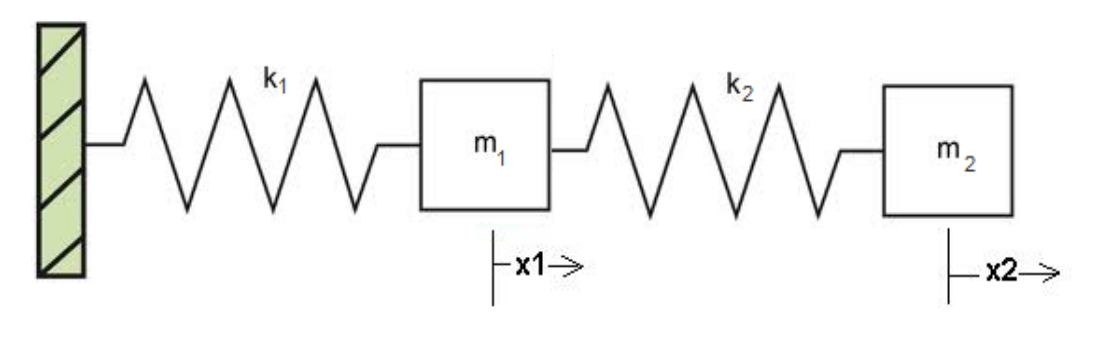
\includegraphics[height=0.2\textwidth,width=0.7\textwidth]{Graphics/mass_spring_system2.png}
     \end{center}
   \end{figure}
   
   Here we have two degrees of freedom that is $x_1$ and $x_2$. The
   velocities of the masses are then $\dot{x_1}$ and $\dot{x_2}$. The
   accelerations are found by doing a free body diagram which results
   in the equations below. The derivation of the equations below are
   left as an exercise to the reader.

   \begin{equation}
     \begin{Bmatrix} \dot{x_1} \\ \ddot{x_1} \\ \dot{x_2}
       \\ \ddot{x_2} \end{Bmatrix}
     = \begin{bmatrix} 0 & 1 & 0 & 0 \\ (-k_1-k_2)/m_1 & 0 & k_2/m_1
       & 0 \\ 0 & 0 & 0 & 1 \\ k_2/m_2 & 0 & -k_2/m_2 & 0 \end{bmatrix} \begin{Bmatrix} x_1 \\ \dot{x_1} \\ x_2
       \\ \dot{x_2} \end{Bmatrix}
   \end{equation}

   This can easily be put into the form $\dot{\vec{x}} =
   A\vec{x}$. The solution to this equation is then simply $\vec{x}(t)
   = e^{At}\vec{x}_0$. Using values $k_1 = k_2 = 200 N/m$ and $m_1 =
   m_2 = 1 kg$ along with initial conditions $\vec{x}_0 = [2,0,0,0]$,
   the solution can be plotted using the MATLAB programming
   language. 
   
   \begin{figure}[htb]
     \begin{center}
       \begin{tabular}{cc}
         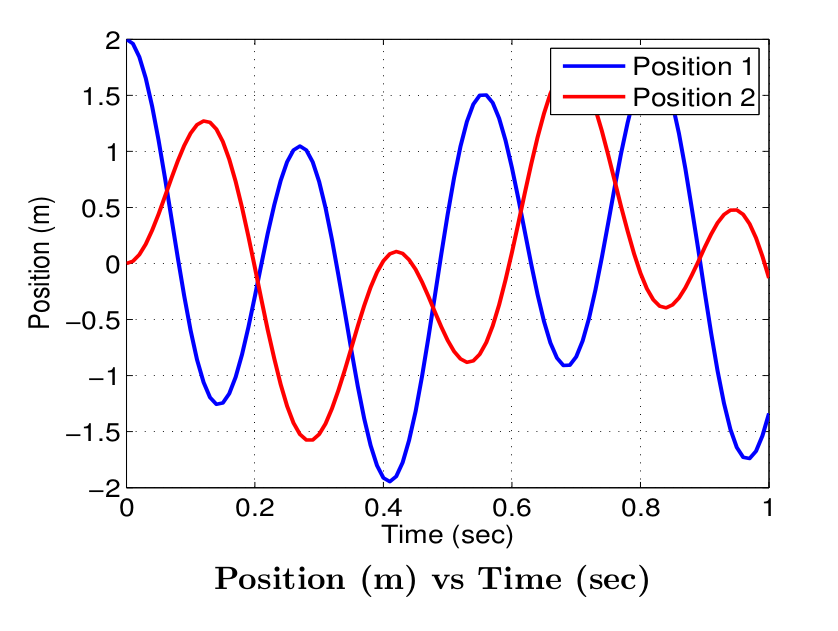
\includegraphics[height=60mm,width=90mm]{Graphics/SpringMassPosition}
         &
         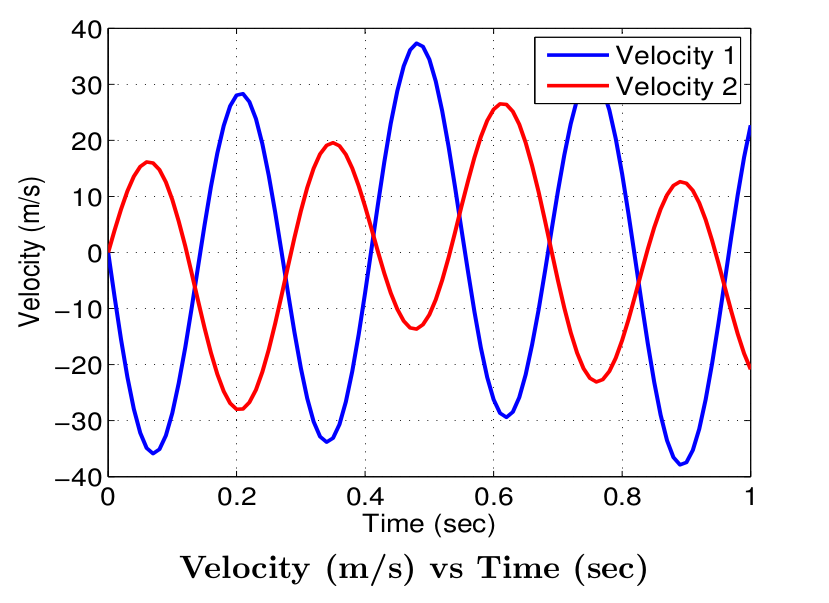
\includegraphics[height=60mm,width=90mm]{Graphics/SpringMassVelocity} \\
                         {\bf Position (m) vs Time (sec)}
                         &
                         {\bf Velocity (m/s) vs Time (sec)}
       \end{tabular}
     \end{center}
   \end{figure}

   The basic code required to plot the solution is shown below.

   \begin{framed}
     x0 = [2;0;0;0];

     k1 = 200;k2 = 200;

     m1 = 1;m2 = 1; 

     A = [0 1 0 0;(-k1-k2)/m1 0 k2/m1 0;0 0 0 1;k2/m2 0 -k2/m2 0]; 

     t = 0:0.01:1; 

     x = zeros(4,length(t)); 

     for idx = 1:length(t) 

     ~~~~x(:,idx) = expm(A.*t(idx))*x0; 

     end 

     plot(t,x) 
   \end{framed}

   This problem can also be solved using the eigenvalue
   solution. Since there are four mode shapes the solution is given by 

   \begin{equation}
     \vec{x}(t) = a_1\vec{v}_1e^{\lambda_1 t} +
     a_2\vec{v}_2e^{\lambda_2 t} + a_3\vec{v}_3e^{\lambda_3 t} +
     a_4\vec{v}_4e^{\lambda_4 t}
   \end{equation}

   The solution to obtaining the eigenvalues and eigenvectors for a
   4x4 matrix by hand is beyond the scope of this course. Thus a
   numerical solver will be used to obtain the eigenvalues and
   eigenvectors. Using the parameters previously defined our A
   matrix is
   
   \begin{equation}
     A = \begin{bmatrix} 0 & 1 & 0 & 0 \\ -400 & 0 & 200
       & 0 \\ 0 & 0 & 0 & 1 \\ 200 & 0 & -200 & 0 \end{bmatrix} 
   \end{equation}

   Using the function $[V,L] = eig(A)$ in MATLAB produces the
   following result 

   \begin{equation}
     L = \begin{bmatrix} 22.9i & 0 & 0 & 0 \\ 0 & -22.9i & 0
       & 0 \\ 0 & 0 & 8.74i & 0 \\ 0 & 0 & 0 & -8.74i \end{bmatrix} 
   \end{equation}

   where the diagonal components are the four eigenvalues. Notice that
   the eigenvalues are actually complex eigenvalues which means there
   are actually only two mode shapes and four eigenvalues. The two
   sets of mode shapes are complex conjugates of each other. The
   $eig()$ function in MATLAB also produces the eigenvectors

   \begin{equation}
     V = \begin{bmatrix} -0.04i & 0.04 & -0.06i & 0.06i \\ 0.85 & 0.85 & 0.52
       & 0.52 \\ 0.02i & -0.02i & -0.10i & 0.10 \\ -0.53 & -0.53 & 0.85 & 0.85 \end{bmatrix} 
   \end{equation}
   
   where each column of the V matrix is an eigenvector of the
   system. Note again that the real components of columns 1 and 2 are
   the same while the imaginary components are different. The same is
   true with columns 3 and 4. The $a$ coefficients are solved by using the formula $\vec{a} =
   V^{-1}\vec{x}_0$. This can also be solved by simply using a
   numerical solver.

   \begin{equation}
     \vec{a} = \begin{Bmatrix} 19.5i \\ -19.5i \\ 4.63i
       \\ -4.63i \end{Bmatrix}
   \end{equation}

   Using these coefficients, eigenvalues and eigenvectors
   it is possible to write the solution of the system. 

   \begin{equation}
     \vec{x}(t) = 19.5i\begin{Bmatrix} -0.04i \\ 0.85 \\ 0.02i \\
     -0.53 \end{Bmatrix} e^{22.9i t} -
     19.5i\begin{Bmatrix} 0.04i \\ 0.85 \\ -0.02i \\
     -0.53 \end{Bmatrix}e^{-22.9i t} + 
     4.63i\begin{Bmatrix} -0.06i \\ 0.52 \\ -0.10i \\
     0.85 \end{Bmatrix} e^{8.74i t} -
     4.63i\begin{Bmatrix} 0.06i \\ 0.52 \\ 0.10i \\
     0.85 \end{Bmatrix}e^{-8.74i t}
   \end{equation}
   
   Remember that if Euler's formula is used the two exponent's will be
   combined to produce $sines$ and $cosines$. Still, this result is
   very powerful because it tells you the two fundamental frequencies
   associated with this system. This solution can also be implemented easily
   in a numerical program such as MATLAB.

   \begin{framed}
     [V,L] = eig(A);

     a = inv(V)*x0;

     xEigen = zeros(4,length(t));

     for idx = 1:length(t)

     ~~~~~~~for n = 1:4

     ~~~~~~~~~~~~xEigen(:,idx) = xEigen(:,idx) + a(n)*V(:,n)*exp(L(n,n)*t(idx));

     ~~~~~~~end

     end

     plot(t,xEigen)
   \end{framed}

\end{enumerate}
